\documentclass[tikz,border=4pt]{standalone}
\usepackage{fontspec}
\usepackage{xcolor}
\usetikzlibrary{arrows.meta,positioning}
\setmainfont{TeX Gyre Pagella}
\setsansfont{Lato}
\definecolor{calm}{HTML}{CDE8DD}
\definecolor{mobilise}{HTML}{F5DEC1}
\definecolor{shutdown}{HTML}{DDE0F0}
\begin{document}
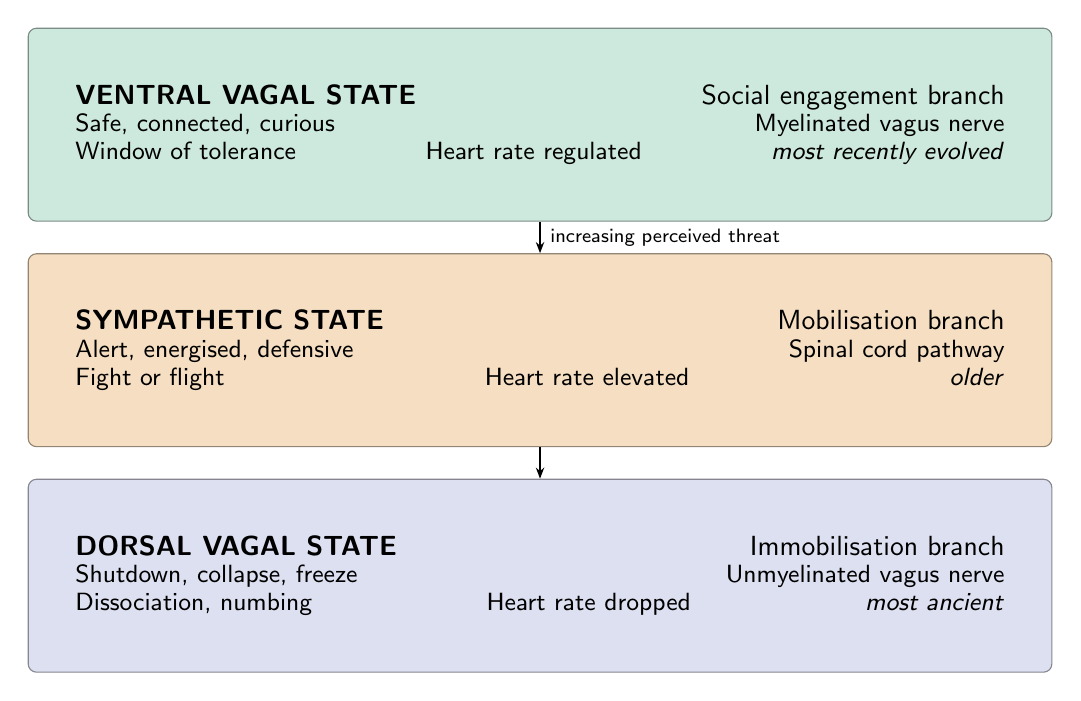
\begin{tikzpicture}[font=\sffamily,box/.style={rounded corners=3pt,draw=#1!60!black,fill=#1,minimum width=13cm,minimum height=2.45cm,inner sep=5mm}]
  \node[box=calm] (ventral) {\begin{minipage}{11.8cm}\textbf{VENTRAL VAGAL STATE}\hfill Social engagement branch\\[-1pt]\small Safe, connected, curious\hfill Myelinated vagus nerve\\[-1pt]\small Window of tolerance\hfill Heart rate regulated\hfill\textit{most recently evolved}\end{minipage}};
  \node[box=mobilise,below=4mm of ventral] (sympathetic) {\begin{minipage}{11.8cm}\textbf{SYMPATHETIC STATE}\hfill Mobilisation branch\\[-1pt]\small Alert, energised, defensive\hfill Spinal cord pathway\\[-1pt]\small Fight or flight\hfill Heart rate elevated\hfill\textit{older}\end{minipage}};
  \node[box=shutdown,below=4mm of sympathetic] (dorsal) {\begin{minipage}{11.8cm}\textbf{DORSAL VAGAL STATE}\hfill Immobilisation branch\\[-1pt]\small Shutdown, collapse, freeze\hfill Unmyelinated vagus nerve\\[-1pt]\small Dissociation, numbing\hfill Heart rate dropped\hfill\textit{most ancient}\end{minipage}};
  \draw[-{Stealth[length=4pt]},line width=.8pt] (ventral.south) -- (sympathetic.north) node[midway,right,font=\scriptsize\sffamily]{increasing perceived threat};
  \draw[-{Stealth[length=4pt]},line width=.8pt] (sympathetic.south) -- (dorsal.north);
\end{tikzpicture}
\end{document}
